\begin{center}
\begin{tabular}{r|rr|rr}
\toprule
 & \multicolumn{2}{c|}{$C=125,\ M=2000$} & \multicolumn{2}{c}{$C=250,\ M=1500$} \\
Depth $d$ & prefix $K$ & minimum $N$ & prefix $K$ & minimum $N$ \\
\midrule
6 & 1000 & 1092 & 1000 & 1220 \\
12 & 1000 & 1103 & 1000 & 1226 \\
25 & 989 & 1239 & 1000 & 1235 \\
50 & 896 & 1212 & 1000 & 1246 \\
100 & 753 & 1201 & 1000 & 1262 \\
250 & 456 & 1323 & 1000 & 1406 \\
500 & 127 & 1179 & 734 & 1500 \\
750 & 0 & -- & 407 & 1500 \\
1000 & 0 & -- & 133 & 1496 \\
\bottomrule
\end{tabular}
\end{center}

Here $K$ is the complete prefix attaining the requested relative
accuracy within the tested family, and $N$ is the smallest common
budget for that prefix. All 18\,000 targets are retained: 12\,495
have certified exact integer minima and 5505 do not reach the tolerance
through their tested maximum. No final target is unresolved. At $C=250$,
13\,371 endpoint attempts require refinement from 3500 to 5000 decimal
working digits; the failed first attempts are retained. These are
evaluation precisions for this certificate, not necessary bit-$P$ limits.

The full unfitted action inversion remains imperfect. At $C=125$,
the 25-digit model misses 14 reachable targets; at 500 digits it
underbudgets 92 of the 127 mutually reachable targets, by as many as
19 modes, and predicts one additional target not reached by $N=2000$.
At $C=250$, the six-digit budget is insufficient at three indices;
at 1000 digits it underbudgets 112 of 133 mutually reachable targets,
by as many as 11 modes. All non-reach outcomes are included in the
comparison. These discrepancies concern the required number of modes,
not the relative error of a displacement predictor.

\begin{figure}[htbp]
\centering
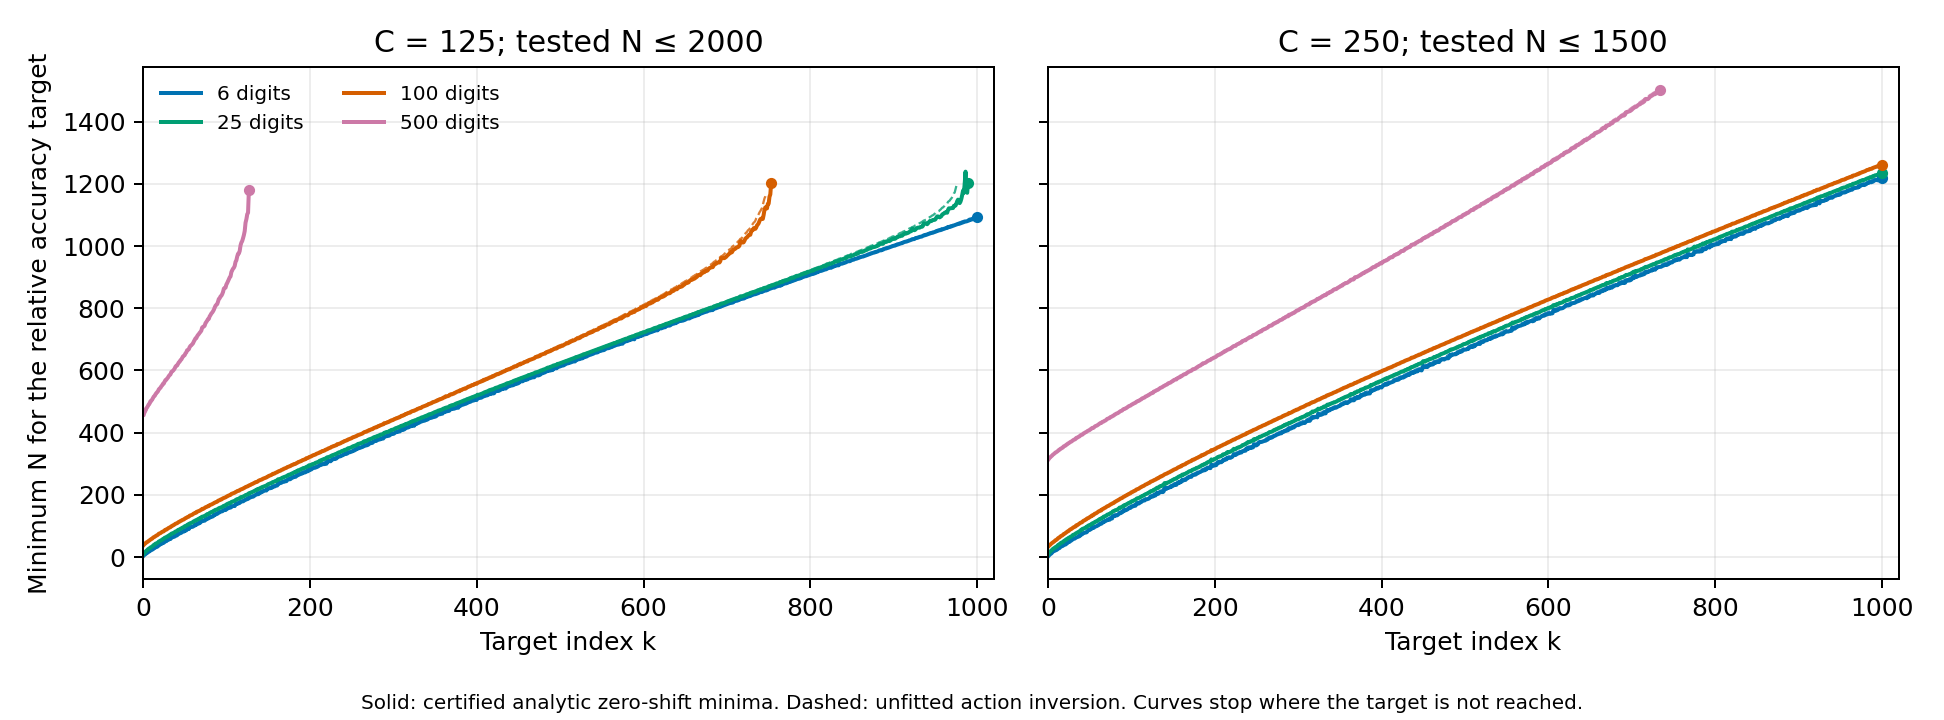
\includegraphics[width=\linewidth]{figures/accuracy_budgets.png}
\caption{Specified-accuracy mode budgets for the finite analytic
zero-shift pencils. The cutoff and requested depth change both the
reachable prefix and its mode requirement. No fixed integer padding
has been fitted.}
\label{fig:accuracy-budgets}
\end{figure}

